%package list
\documentclass{article}
\usepackage[top=3cm, bottom=3cm, outer=3cm, inner=3cm]{geometry}
\usepackage{multicol}
\usepackage{graphicx}
\usepackage{url}
%\usepackage{cite}
\usepackage{hyperref}
\usepackage{array}
%\usepackage{multicol}
\newcolumntype{x}[1]{>{\centering\arraybackslash\hspace{0pt}}p{#1}}
\usepackage{natbib}
\usepackage{pdfpages}
\usepackage{multirow}
\usepackage[normalem]{ulem}
\useunder{\uline}{\ul}{}
\usepackage{svg}
\usepackage{xcolor}
\usepackage{listings}
\lstdefinestyle{ascii-tree}{
    literate={├}{|}1 {─}{--}1 {└}{+}1 
  }
\lstset{basicstyle=\ttfamily,
  showstringspaces=false,
  commentstyle=\color{red},
  keywordstyle=\color{blue}
}
%\usepackage{booktabs}
\usepackage{caption}
\usepackage{subcaption}
\usepackage{float}
\usepackage{array}

\newcolumntype{M}[1]{>{\centering\arraybackslash}m{#1}}
\newcolumntype{N}{@{}m{0pt}@{}}


%%%%%%%%%%%%%%%%%%%%%%%%%%%%%%%%%%%%%%%%%%%%%%%%%%%%%%%%%%%%%%%%%%%%%%%%%%%%
%%%%%%%%%%%%%%%%%%%%%%%%%%%%%%%%%%%%%%%%%%%%%%%%%%%%%%%%%%%%%%%%%%%%%%%%%%%%
\newcommand{\itemEmail}{rvaldiviase@unsa.edu.pe}
\newcommand{\itemStudent}{Ryan Fabian Valdivia Segovia}
\newcommand{\itemCourse}{Fundamentos de la programación 2}
\newcommand{\itemCourseCode}{1701213}
\newcommand{\itemSemester}{II}
\newcommand{\itemUniversity}{Universidad Nacional de San Agustín de Arequipa}
\newcommand{\itemFaculty}{Facultad de Ingeniería de Producción y Servicios}
\newcommand{\itemDepartment}{Departamento Académico de Ingeniería de Sistemas e Informática}
\newcommand{\itemSchool}{Escuela Profesional de Ingeniería de Sistemas}
\newcommand{\itemAcademic}{2023 - B}
\newcommand{\itemInput}{Del 18 Septiembre 2023}
\newcommand{\itemOutput}{Al 24 Septiembre 2023}
\newcommand{\itemPracticeNumber}{03}
\newcommand{\itemTheme}{Arreglos de objetos}
%%%%%%%%%%%%%%%%%%%%%%%%%%%%%%%%%%%%%%%%%%%%%%%%%%%%%%%%%%%%%%%%%%%%%%%%%%%%
%%%%%%%%%%%%%%%%%%%%%%%%%%%%%%%%%%%%%%%%%%%%%%%%%%%%%%%%%%%%%%%%%%%%%%%%%%%%

\usepackage[english,spanish]{babel}
\usepackage[utf8]{inputenc}
\AtBeginDocument{\selectlanguage{spanish}}
\renewcommand{\figurename}{Figura}
\renewcommand{\refname}{Referencias}
\renewcommand{\tablename}{Tabla} %esto no funciona cuando se usa babel
\AtBeginDocument{%
	\renewcommand\tablename{Tabla}
}

\usepackage{fancyhdr}
\pagestyle{fancy}
\fancyhf{}
\setlength{\headheight}{30pt}
\renewcommand{\headrulewidth}{1pt}
\renewcommand{\footrulewidth}{1pt}
\fancyhead[L]{\raisebox{-0.2\height}{
\includegraphics[width=3cm]{img/logo_episunsa.png}}}
\fancyhead[C]{\fontsize{7}{7}\selectfont	\itemUniversity \\ \itemFaculty \\ \itemDepartment \\ \itemSchool \\ \textbf{\itemCourse}}
\fancyhead[R]{\raisebox{-0.2\height}{
\includegraphics[width=1.2cm]{img/logo_abet}}}
\fancyfoot[L]{Estudiante Ryan Valdivia}
\fancyfoot[C]{\itemCourse}
\fancyfoot[R]{Página \thepage}

% para el codigo fuente
\usepackage{listings}
\usepackage{color, colortbl}
\definecolor{dkgreen}{rgb}{0,0.6,0}
\definecolor{gray}{rgb}{0.5,0.5,0.5}
\definecolor{mauve}{rgb}{0.58,0,0.82}
\definecolor{codebackground}{rgb}{0.95, 0.95, 0.92}
\definecolor{tablebackground}{rgb}{0.8, 0, 0}

\lstset{frame=tb,
	language=bash,
	aboveskip=3mm,
	belowskip=3mm,
	showstringspaces=false,
	columns=flexible,
	basicstyle={\small\ttfamily},
	numbers=none,
	numberstyle=\tiny\color{gray},
	keywordstyle=\color{blue},
	commentstyle=\color{dkgreen},
	stringstyle=\color{mauve},
	breaklines=true,
	breakatwhitespace=true,
	tabsize=3,
	backgroundcolor= \color{codebackground},
}

\begin{document}
	
	\vspace*{10px}
	
	\begin{center}	
		\fontsize{17}{17} \textbf{ Informe de Laboratorio \itemPracticeNumber}
	\end{center}
	\centerline{\textbf{\Large Tema: \itemTheme}}
	%\vspace*{0.5cm}	

	\begin{flushright}
		\begin{tabular}{|M{2.5cm}|N|}
			\hline 
			\rowcolor{tablebackground}
			\color{white} \textbf{Nota}  \\
			\hline 
			     \\[30pt]
			\hline 			
		\end{tabular}
	\end{flushright}	

	\begin{table}[H]
		\begin{tabular}{|x{4.7cm}|x{4.8cm}|x{4.8cm}|}
			\hline 
			\rowcolor{tablebackground}
			\color{white} \textbf{Estudiante} & \color{white}\textbf{Escuela}  & \color{white}\textbf{Asignatura}   \\
			\hline 
			{\itemStudent \par \itemEmail} & \itemSchool & {\itemCourse \par Semestre: \itemSemester \par Código: \itemCourseCode}     \\
			\hline 			
		\end{tabular}
	\end{table}		
	
	\begin{table}[H]
		\begin{tabular}{|x{4.7cm}|x{4.8cm}|x{4.8cm}|}
			\hline 
			\rowcolor{tablebackground}
			\color{white}\textbf{Laboratorio} & \color{white}\textbf{Tema}  & \color{white}\textbf{Duración}   \\
			\hline 
			\itemPracticeNumber & \itemTheme & 04 horas   \\
			\hline 
		\end{tabular}
	\end{table}
	
	\begin{table}[H]
		\begin{tabular}{|x{4.7cm}|x{4.8cm}|x{4.8cm}|}
			\hline 
			\rowcolor{tablebackground}
			\color{white}\textbf{Semestre académico} & \color{white}\textbf{Fecha de inicio}  & \color{white}\textbf{Fecha de entrega}   \\
			\hline 
			\itemAcademic & \itemInput &  \itemOutput  \\
			\hline 
		\end{tabular}
	\end{table}
	
	\section{Tarea}
	\begin{itemize}
		\subsection{Actividad 1: Demo Batalla}
			\item Analice, complete y pruebe el Código de la clase DemoBatalla.
		\subsection{Actividad 2}
			\item Solucionar la Actividad 4 de la Práctica 1 pero usando arreglo de objetos.
		\subsection{Actividad 3}
			\item Solucionar la Actividad 5 de la Práctica 1 pero usando arreglos de objetos.
	\end{itemize}
		
	\section{Equipos, materiales y temas utilizados}
	\begin{itemize}
		\item Sistema Operativo Windows 11 Home Single Language 64 bits 22621.2283
		\item VIM 9.0.
		\item Visual Studio Code 64 bits 1.82.2
		\item OpenJDK 64-Bits 11.0.16.1
		\item Git 2.41.0.windows.1
		\item Cuenta en GitHub con el correo institucional. 
		\item Código parcial proporcionado por el profesor.
	\end{itemize}
	
	\section{URL de Repositorio Github}
	\begin{itemize}
		\item URL del Repositorio GitHub para clonar o recuperar.
		\item \url{https://github.com/RyanValdivia/fp2-23b.git}
		\item URL para el laboratorio 03 en el Repositorio GitHub.
		\item \url{https://github.com/RyanValdivia/fp2-23b/tree/main/fase01/lab03}
	\end{itemize}
	
	\section{Actividades}
	\subsection{Actividad 1}
	
	\begin{itemize}	
		\item Realicé un commit copiando el código parcial que nos proporcionó el profesor.
	\end{itemize}	
	\begin{lstlisting}[language=bash,caption={Comentando el código paricial}][H]
		$ git log Ahorcado.java
		commit b1ca8e2e60d9546da50d357333768c59ebeb0135
		Author: RYAN VALDIVIA <rvaldiviase@unsa.edu.pe>
		Date:   Sun Sep 24 14:36:27 2023 -0500
			Actividad 1: Copiando el codigo parcial que nos dio el profesor
	\end{lstlisting}
	\begin{lstlisting}[language=java,caption={Código parcial de DemoBatalla}, numbers=left][H]
import java.util.*;

public class DemoBatalla {
    public static void main(String[] args) {
        Nave[] misNaves = new Nave[10];
        Scanner sc = new Scanner(System.in);
        String nomb, col;
        int fil, punt;
        boolean est;
        for (int i = 0; i < misNaves.length; i++) {
            System.out.println("Nave " + (i + 1));
            System.out.println("Nombre: ");
            nomb = sc.next();
            System.out.println("Fila ");
            fil = sc.nextInt();
            System.out.println("Columna: ");
            col = sc.next();
            System.out.println("Estado: ");
            est = sc.nextBoolean();
            System.out.println("Puntos: ");
            punt = sc.nextInt();
            misNaves[i] = new Nave(); // Se crea un objeto Nave y se asigna su referencia a misNaves
            misNaves[i].setNombre(nomb);
            misNaves[i].setFila(fil);
            misNaves[i].setColumna(col);
            misNaves[i].setEstado(est);
            misNaves[i].setPuntos(punt);
        }
        System.out.println("\nNaves creadas:");
        mostrarNaves(misNaves);
        mostrarPorNombre(misNaves);
        mostrarPorPuntos(misNaves);
        System.out.println("\nNave con mayor numero de puntos: " + mostrarMayorPuntos(misNaves));
    }

    // Metodo para mostrar todas las naves
    public static void mostrarNaves(Nave[] flota) {
    }

    // Metodo para mostrar todas las naves de un nombre que se pide por teclado
    public static void mostrarPorNombre(Nave[] flota) {
    }

    // Metodo para mostrar todas las naves con un numero de puntos inferior o igual
    // al numero de puntos que se pide por teclado
    public static void mostrarPorPuntos(Nave[] flota) {
    }

    // Metodo que devuelve la Nave con mayor numero de Puntos
    public static Nave mostrarMayorPuntos(Nave[] flota) {
    }
    // Crear un metodo que devuelva un nuevo arreglo de objetos con todos los
    // objetos previamente ingresados
    // pero aleatoriamente desordenados
}
	\end{lstlisting}
	\begin{itemize}	
		\item También tenemos el código de la clase auxiliar Nave. 
	\end{itemize}
	\begin{lstlisting}[language=java,caption={Clase Nave}, numbers=left][H]
public class Nave {
    private String nombre;
    private int fila;
    private String columna;
    private boolean estado;
    private int puntos;

    // Metodos mutadores
    public void setNombre(String n) {
        nombre = n;
    }

    public void setFila(int f) {
        fila = f;
    }

    public void setColumna(String c) {
        columna = c;
    }

    public void setEstado(boolean e) {
        estado = e;
    }

    public void setPuntos(int p) {
        puntos = p;
    }

    // Metodos accesores
    public String getNombre() {
        return nombre;

    }

    public int getFila() {
        return fila;

    }

    public String getColumna() {
        return columna;

    }

    public boolean getEstado() {
        return estado;

    }

    public int getPuntos() {
        return puntos;

    }
    // Completar con otros metodos necesarios
}
	\end{lstlisting}
	\begin{itemize}	
		\item Lo primero que hice fue elaborar el método de mostrarNaves, haciendo que simplemente se impriman todas las naves del arreglo junto con sus respectivos atributos, usando un ciclo for each para recorrer el arreglo.
	\end{itemize}
	\begin{lstlisting}[language=java,caption={Mostrar naves}, numbers=left][H]
	public static void mostrarNaves(Nave[] flota) {
        int i = 1;
        for (Nave n : flota) {
            System.out.println("Nave " + i + ":" + n.getNombre());
            System.out.println("Posicion: " + n.getFila() + n.getColumna());
            System.out.println("Puntos: " + n.getPuntos());
            if (n.getEstado()) {
                System.out.println("Sigue con vida");
            } else {
                System.out.println("Fue destruido");
            }
            System.out.println();
            i++;
        }
    }
	\end{lstlisting}
	\begin{itemize}	
		\item La razón por la trabajé este método primero, fue para usarlo de base para los siguientes métodos.
		\item Para el método de mostrarPorNombre, seguí la lógica del método anterior, con la modificación de mostrar solo las naves que coincidan con el nombre que ingrese el usuario.
	\end{itemize}
	\begin{lstlisting}[language=java,caption={Mostrar por Nombre}, numbers=left][H]
	public static void mostrarPorNombre(Nave[] flota) {
        Scanner sc = new Scanner(System.in);
        String nombre = sc.next();
        for (int i = 0; i < flota.length; i++) {
            if (flota[i].getNombre().equals(nombre)) {
                Nave n = flota[i];
                System.out.println(n.getNombre());
                System.out.println("Posicion: " + n.getFila() + n.getColumna());
                System.out.println("Puntos: " + n.getPuntos());
                if (n.getEstado()) {
                    System.out.println("Sigue con vida");
                } else {
                    System.out.println("Fue destruido");
                }
            }
        }
    }
	\end{lstlisting}
	\begin{itemize}	
		\item Para el siguiente método, continué con la lógica, solo modificando el ciclo con un condicional para imprimir las naves que tengan un puntaje menor o igual al ingresado por teclado.
	\end{itemize}
	\begin{lstlisting}[language=java,caption={Mostrando por puntos menores o iguales}, numbers=left][H]
	public static void mostrarPorPuntos(Nave[] flota) {
        Scanner sc = new Scanner(System.in);
        int puntos = sc.nextInt();
        for (int i = 0; i < flota.length; i++) {
            if (flota[i].getPuntos() <= puntos) {
                Nave n = flota[i];
                System.out.println("Nave " + i + ":" + n.getNombre());
                System.out.println("Posicion: " + n.getFila() + n.getColumna());
                System.out.println("Puntos: " + n.getPuntos());
                if (n.getEstado()) {
                    System.out.println("Sigue con vida");
                } else {
                    System.out.println("Fue destruido");
                }
            }
        }
    }
	\end{lstlisting}
	\begin{itemize}	
		\item El siguiente método es un algoritmo conocido y simple para saber cual es el objeto de mayor valor en un arreglo, lo usé para el método de mostrarMayorPuntos.
	\end{itemize}
	\begin{lstlisting}[language=java,caption={Mostrar la nave con mayor cantidad de puntos}, numbers=left][H]
	public static Nave mostrarMayorPuntos(Nave[] flota) {
        int mayor = 0;
        for (int i = 0; i < flota.length; i++) {
            if (flota[i].getPuntos() > flota[mayor].getPuntos()) {
                mayor = i;
            }
        }
        return flota[mayor];
    }
	\end{lstlisting}	
	\begin{itemize}	
		\item Finalmente, se viene algo un poco más complicado, el método para desordenar el arreglo de naves, para hacer esto, hice dos métodos auxiliares.
		\item En primer lugar, mi estrategia fue crear un arreglo de enteros conteniendo los numeros del 0 a la longitud del arreglo de naves (En este caso, 10), y usarlo para desordenar el arreglo.
	\end{itemize}
	\begin{lstlisting}[language=java,caption={Método para obtener números desordenados}, numbers=left][H]
	 public static int[] numerosRandom(Nave[] flota) {
        int[] nums = new int[flota.length];
        for (int i = 0; i < nums.length; i++) {
            nums[i] = nums.length;
        }
        for (int i = 0; i < flota.length; i++) {
            int n;
            do {
                n = (int) (Math.random() * flota.length);
            } while (estaEnArreglo(nums, n, i));
            nums[i] = n;
        }
        return nums;
    }
	\end{lstlisting}
	\begin{itemize}	
		\item Y para esto, necesitaba una forma de comprobar que el número aleatorio que generé no estuviera antes en el arreglo, para que no haya números repetidos, por tanto, creé el método estaEnArreglo para hacer esa comprobación.
	\end{itemize}
	\begin{lstlisting}[language=java,caption={Método está en Arreglo}, numbers=left][H]
	 public static boolean estaEnArreglo(int[] arreglo, int num, int indice) {
        for (int i = 0; i < indice; i++) {
            if (arreglo[i] == num) {
                return true;
            }
        }
        return false;
    }
	\end{lstlisting}
	\begin{itemize}	
		\item Con el arreglo de números aleatorios ya hecho, solo me queda armar todo para desordenar un arreglo de naves dado.
	\end{itemize}
	\begin{lstlisting}[language=java,caption={Desordenar arreglo}, numbers=left][H]
	 public static Nave[] desordenar(Nave[] flota) {
        Nave[] desordenado = new Nave[flota.length];
        int[] desorden = numerosRandom(flota);
        for (int i = 0; i < desordenado.length; i++) {
            desordenado[i] = flota[desorden[i]];
        }
        return desordenado;
    }
	\end{lstlisting}
	\begin{itemize}	
		\item Solo me falta añadir un par de cosas en el método main para que funcione al 100%.
	\end{itemize}
	\begin{lstlisting}[language=java,caption={Método main}, numbers=left][H]
	 System.out.println("\nNave con mayor numero de puntos: " + mostrarMayorPuntos(misNaves).getNombre());
        mostrarNaves(desordenar(misNaves));
	\end{lstlisting}
	\begin{itemize}	
		\item Con esto ya tengo el código de DemoBatalla listo para su uso.
		\item A continuación tengo algunas capturas de la ejecución del código, usando solo cinco naves en el arreglo para no tener que introducir tantos datos.
	\end{itemize}
	\begin{itemize}
		\item Llenando los datos del arreglo.
	\end{itemize}

	\begin{figure}[H]
		\centering		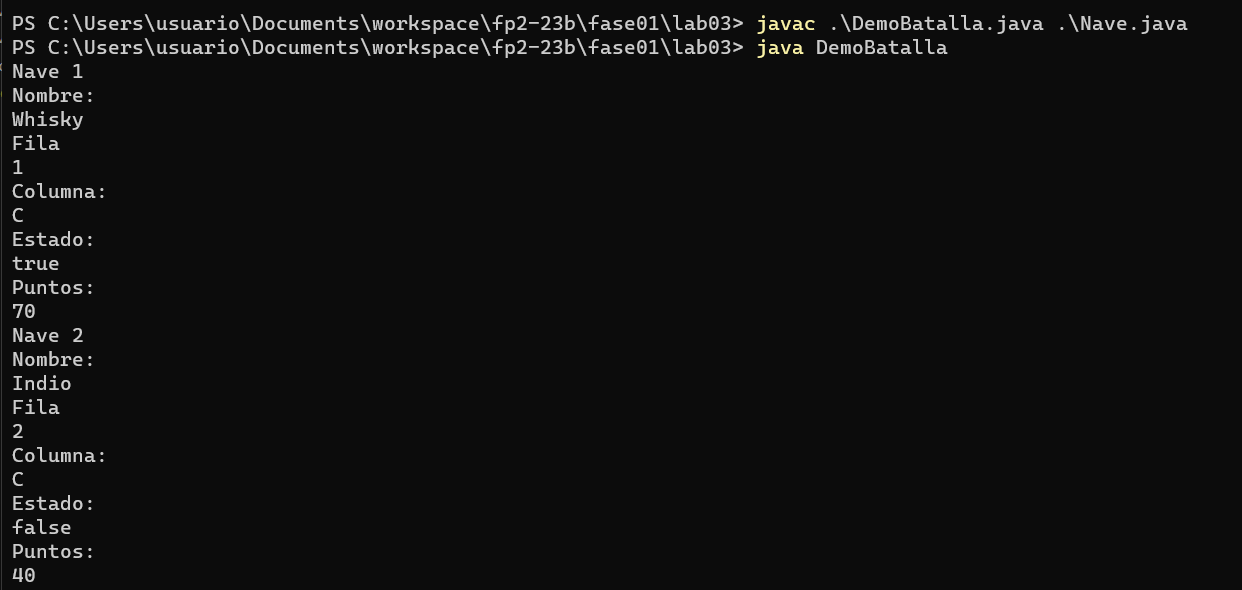
\includegraphics[width=0.8\textwidth,keepaspectratio]{img/captura1.png}
		%\includesvg{img/automata.svg}
		%\label{img:mot2}
		%\caption{Product backlog.}
	\end{figure}
	
	\begin{figure}[H]
		\centering
	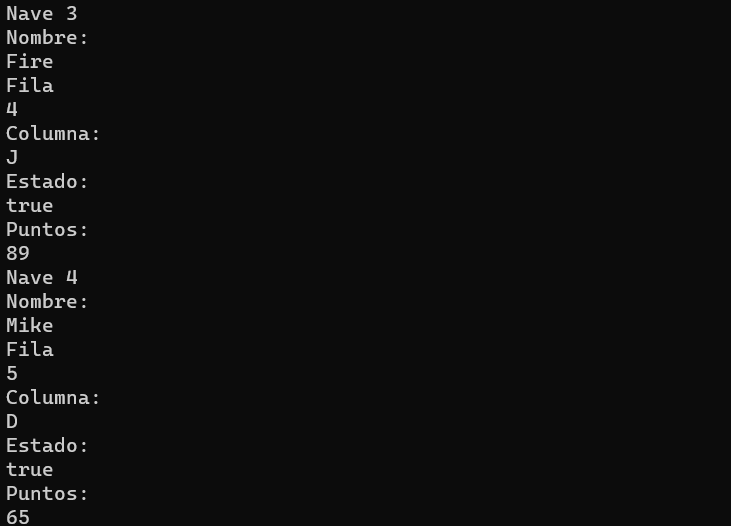
\includegraphics[width=0.8\textwidth,keepaspectratio]{img/captura2.png}
		%\includesvg{img/automata.svg}
		%\label{img:mot2}
		%\caption{Product backlog.}
	\end{figure}
	
	\begin{figure}[H]
		\centering
	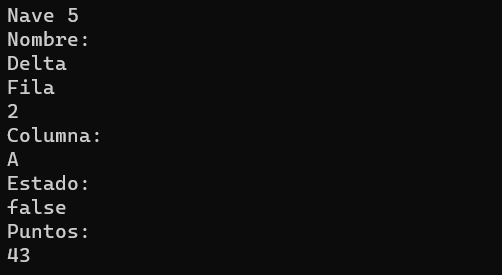
\includegraphics[width=0.5\textwidth,keepaspectratio]{img/captura3.png}
		%\includesvg{img/automata.svg}
		%\label{img:mot2}
		%\caption{Product backlog.}
	\end{figure}
	
	\begin{itemize}
		\item Probando el método para mostrar todas las naves.
	\end{itemize}
	\begin{figure}[H]
		\centering
	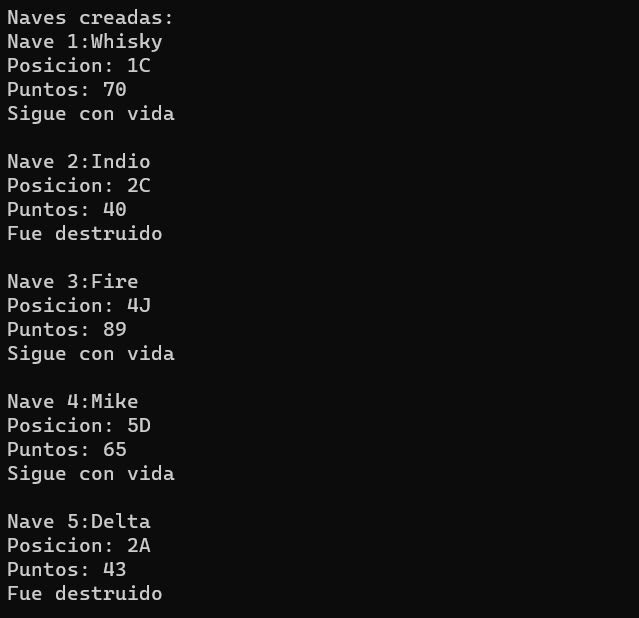
\includegraphics[width=0.8\textwidth,keepaspectratio]{img/captura4.png}
		%\includesvg{img/automata.svg}
		%\label{img:mot2}
		%\caption{Product backlog.}
	\end{figure}
	
	\begin{itemize}
		\item Probando el método para búsqueda por nombre.
	\end{itemize}
	\begin{figure}[H]
		\centering
	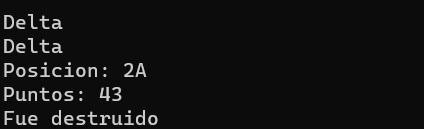
\includegraphics[width=0.8\textwidth,keepaspectratio]{img/captura5.png}
		%\includesvg{img/automata.svg}
		%\label{img:mot2}
		%\caption{Product backlog.}
	\end{figure}
	
	\begin{itemize}
		\item Probando el método para búsqueda por puntos.
	\end{itemize}
	\begin{figure}[H]
		\centering
	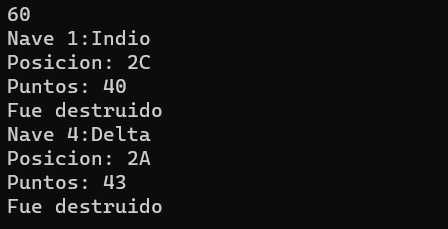
\includegraphics[width=0.8\textwidth,keepaspectratio]{img/captura6.png}
		%\includesvg{img/automata.svg}
		%\label{img:mot2}
		%\caption{Product backlog.}
	\end{figure}
	
	\begin{itemize}
		\item Probando el método para saber la Nave con mayor puntuación.
	\end{itemize}
	\begin{lstlisting}[language=bash,caption={Nave con el puntaje más alto}][H]
		Nave con mayor numero de puntos: Fire
	\end{lstlisting}
	
	\begin{itemize}
		\item Probando el método para desordenar todas las naves aleatoriamente y luego mostrarlas.
	\end{itemize}
	\begin{figure}[H]
		\centering
	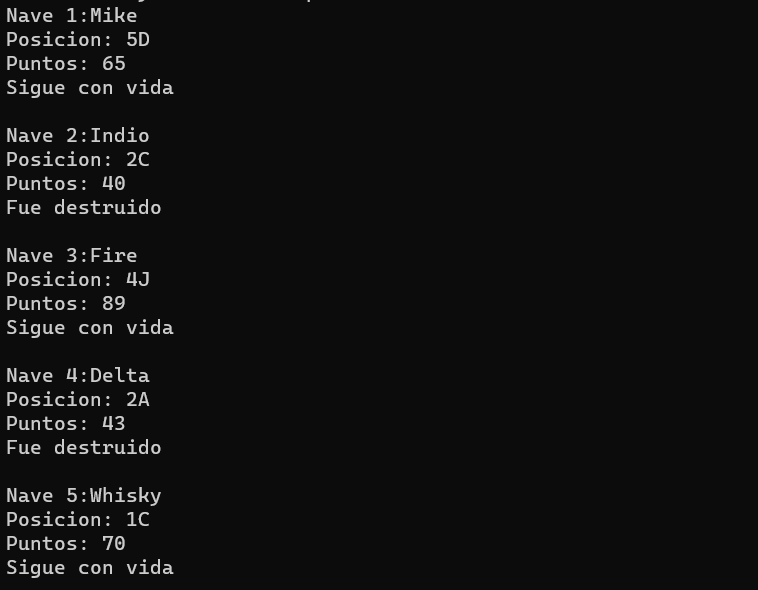
\includegraphics[width=0.8\textwidth,keepaspectratio]{img/captura7.png}
		%\includesvg{img/automata.svg}
		%\label{img:mot2}
		%\caption{Product backlog.}
	\end{figure}
	
	\subsection{Actividad 2}
	\begin{itemize}
		\item Para poder trabajar con arreglos de objetos en esta actividad y la siguiente, necesito crear una clase conveniente, en este caso, creé la clase 'Soldado' con sus atributos respectivos.
	\end{itemize}
	
	\begin{lstlisting}[language=java,caption={Clase Soldado}, numbers=left][H]
public class Soldado {
    private String nombre;
    private int vida;

    public void setNombre(String s) {
        this.nombre = s;
    }

    public void setVida(int n) {
        this.vida = n;
    }

    public String getNombre() {
        return nombre;
    }

    public int getVida() {
        return vida;
    }
}
	\end{lstlisting}
	
	\begin{itemize}
		\item Ahora simplemente trabajé la actividad de leer los nombres y niveles de vida de cinco soldados, usando un arreglo de 'Soldados'.
		\item Para esto, almaceno los valores como atributos de los objetos Soldado, como la vida y el nombre.
	\end{itemize}
	\begin{lstlisting}[language=java,caption={Los 5 soldados}, numbers=left][H]
import java.util.*;

public class VideoJuego {
    public static void main(String[] args) {
        Scanner sc = new Scanner(System.in);
        Soldado[] army = new Soldado[5];
        for (int i = 0; i < army.length; i++) {
            army[i] = new Soldado();
            System.out.println("Ingrese el nombre del soldado: ");
            army[i].setNombre(sc.next());
            System.out.println("Ingrese su nivel de vida");
            army[i].setVida(sc.nextInt());
        }
        int i = 1;
        for (Soldado s : army) {
            System.out.println("Soldado " + i + " : " + s.getNombre());
            System.out.println("Tiene " + s.getVida() + " puntos de vida\n");
            i++;
        }
    }
}
	\end{lstlisting}
	
	\begin{itemize}
		\item Y ahora trabajo el problema de los dos ejércitos usando arreglos de objetos, la lógica es similar pero para almacenar los nombres uso los atributos de los objetos.
	\end{itemize}
	\begin{lstlisting}[language=java,caption={Los 5 soldados}, numbers=left][H]
public class VideoJuego {
    public static void main(String[] args) {
        int len1 = (int) (Math.random() * 5 + 1);
        int len2 = (int) (Math.random() * 5 + 1);
        Soldado[] army1 = new Soldado[len1];
        Soldado[] army2 = new Soldado[len2];
        init(army1);
        init(army2);
        mostrar(army1, army2);
        win(len1, len2);

    }

    public static void init(Soldado[] soldiers) {
        for (int i = 0; i < soldiers.length; i++) {
            soldiers[i] = new Soldado();
            soldiers[i].setNombre("Soldado " + i);
        }
    }

    public static void win(int l1, int l2) {
        if (l1 > l2) {
            System.out.println("El ejercito 1 es ganador");
        } else if (l1 == l2) {
            System.out.println("Hay empate");
        } else {
            System.out.println("El ejercito 2 es ganador");
        }
    }

    public static void mostrar(Soldado[] army1, Soldado[] army2) {
        System.out.println("Ejercito 1: ");
        for (int i = 0; i < army1.length; i++) {
            System.out.println(army1[i].getNombre());
        }
        System.out.println();
        System.out.println("Ejercito 2: ");
        for (int i = 0; i < army2.length; i++) {
            System.out.println(army2[i].getNombre());
        }

    }
}
	\end{lstlisting}
	
	
	
	\section{\textcolor{red}{Rúbricas}}
	
	\subsection{\textcolor{red}{Entregable Informe}}
	\begin{table}[H]
		\caption{Tipo de Informe}
		\setlength{\tabcolsep}{0.5em} % for the horizontal padding
		{\renewcommand{\arraystretch}{1.5}% for the vertical padding
		\begin{tabular}{|p{3cm}|p{12cm}|}
			\hline
			\multicolumn{2}{|c|}{\textbf{\textcolor{red}{Informe}}}  \\
			\hline 
			\textbf{\textcolor{red}{Latex}} & \textcolor{blue}{El informe está en formato PDF desde Latex,  con un formato limpio (buena presentación) y facil de leer.}   \\ 
			\hline 
			
			
		\end{tabular}
	}
	\end{table}
	
	\clearpage
	
	\subsection{\textcolor{red}{Rúbrica para el contenido del Informe y demostración}}
	\begin{itemize}			
		\item El alumno debe marcar o dejar en blanco en celdas de la columna \textbf{Checklist} si cumplio con el ítem correspondiente.
		\item Si un alumno supera la fecha de entrega,  su calificación será sobre la nota mínima aprobada, siempre y cuando cumpla con todos lo items.
		\item El alumno debe autocalificarse en la columna \textbf{Estudiante} de acuerdo a la siguiente tabla:
	
		\begin{table}[ht]
			\caption{Niveles de desempeño}
			\begin{center}
			\begin{tabular}{ccccc}
    			\hline
    			 & \multicolumn{4}{c}{Nivel}\\
    			\cline{1-5}
    			\textbf{Puntos} & Insatisfactorio 25\%& En Proceso 50\% & Satisfactorio 75\% & Sobresaliente 100\%\\
    			\textbf{2.0}&0.5&1.0&1.5&2.0\\
    			\textbf{4.0}&1.0&2.0&3.0&4.0\\
    		\hline
			\end{tabular}
		\end{center}
	\end{table}	
	
	\end{itemize}
	
	\begin{table}[H]
		\caption{Rúbrica para contenido del Informe y demostración}
		\setlength{\tabcolsep}{0.5em} % for the horizontal padding
		{\renewcommand{\arraystretch}{1.5}% for the vertical padding
		%\begin{center}
		\begin{tabular}{|p{2.7cm}|p{7cm}|x{1.3cm}|p{1.2cm}|p{1.5cm}|p{1.1cm}|}
			\hline
    		\multicolumn{2}{|c|}{Contenido y demostración} & Puntos & Checklist & Estudiante & Profesor\\
			\hline
			\textbf{1. GitHub} & Hay enlace URL activo del directorio para el  laboratorio hacia su repositorio GitHub con código fuente terminado y fácil de revisar. &2 &X &2 & \\ 
			\hline
			\textbf{2. Commits} &  Hay capturas de pantalla de los commits más importantes con sus explicaciones detalladas. (El profesor puede preguntar para refrendar calificación). &4 &X &2 & \\ 
			\hline 
			\textbf{3. Código fuente} &  Hay porciones de código fuente importantes con numeración y explicaciones detalladas de sus funciones. &2 &X &2 & \\ 
			\hline 
			\textbf{4. Ejecución} & Se incluyen ejecuciones/pruebas del código fuente  explicadas gradualmente. &2 &X &2 & \\ 
			\hline			
			\textbf{5. Pregunta} & Se responde con completitud a la pregunta formulada en la tarea.  (El profesor puede preguntar para refrendar calificación).  &2 &X &2 & \\ 
			\hline	
			\textbf{6. Fechas} & Las fechas de modificación del código fuente estan dentro de los plazos de fecha de entrega establecidos. &2 &X &2 & \\ 
			\hline 
			\textbf{7. Ortografía} & El documento no muestra errores ortográficos. &2 &X &2 & \\ 
			\hline 
			\textbf{8. Madurez} & El Informe muestra de manera general una evolución de la madurez del código fuente,  explicaciones puntuales pero precisas y un acabado impecable.   (El profesor puede preguntar para refrendar calificación).  &4 &X &4 & \\ 
			\hline
			\multicolumn{2}{|c|}{\textbf{Total}} &20 & &18 & \\ 
			\hline
		\end{tabular}
		%\end{center}
		%\label{tab:multicol}
		}
	\end{table}
	
\clearpage

\section{Referencias}
	\begin{itemize}
		\item \url {https://www.w3schools.com/java/java_modifiers.asp}
		\item \url {https://puntocomnoesunlenguaje.blogspot.com/2013/04/llenar-un-array-con-numeros-aleatorios.html}
	\end{itemize}
	
%\clearpage
%\bibliographystyle{apalike}
%\bibliographystyle{IEEEtranN}
%\bibliography{bibliography}
			
\end{document}